\documentclass{article}
\usepackage{amsmath}
\usepackage{amssymb}
\usepackage{graphicx}
\usepackage{hyperref}
\usepackage[version=4]{mhchem}

\title{Problem 10}
\date{}

\begin{document}
\maketitle

\section*{Problem}
In trapezoid \(A B C D, A B=3 C D\) and \(A B / / C D\). \(E\) is the midpoint of the diagonal \(A C\). \(B E\) meets \(A D\) at \(F\). Find the value of \(A F\) : \(F D\).\\
(A) \(\frac{5}{3}\)\\
(B) \(\frac{3}{2}\)\\
(C) \(\frac{10}{7}\)\\
(D)\\
(E) \(\frac{12}{5}\).\\
\centering
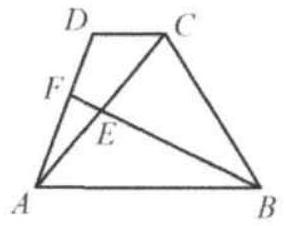
\includegraphics[width=\textwidth]{images/128.jpg}

\section*{Solution}
(B).
Method 1:\\
Extend \(C D\) and \(B F\) to meet at \(G\). Since \(C G / / A B, \triangle A B E\) \(\sim \triangle C G E\). So\\
\centering
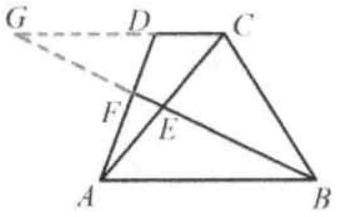
\includegraphics[width=\textwidth]{images/135.jpg}\\
\(\frac{C G}{A B}=\frac{C E}{A E}=1 \Rightarrow C G=A B \Rightarrow\)\\
\(G D+C D=3 C D \Rightarrow G D=2 C D\)\\
Since \(D G / / A B, \triangle A B F \sim \triangle D G E\).\\
\centering
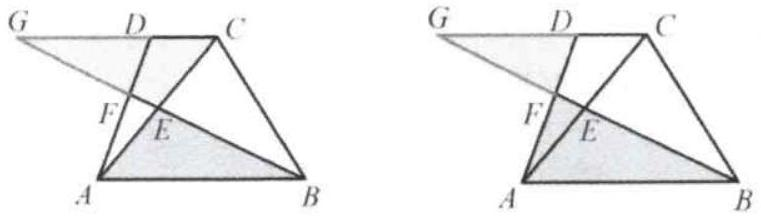
\includegraphics[width=\textwidth]{images/135(1).jpg}


So\\
\(\frac{A F}{F D}=\frac{A B}{D G} \quad \Rightarrow \frac{A F}{F D}=\frac{3 C D}{2 C D}=\frac{3}{2}\).

Method 2:\\
Draw \(C G / / B F\) to meet the extension of \(A D\) at \(G\). Since \(A B / / C D, C G / / B F\),

\[
\begin{aligned}
\triangle A B F & \sim \triangle D C G . \text { So } \frac{A F}{D G}=\frac{A B}{C D}=3 \\
& \Rightarrow A F=3 D G .
\end{aligned}
\]

\begin{center}
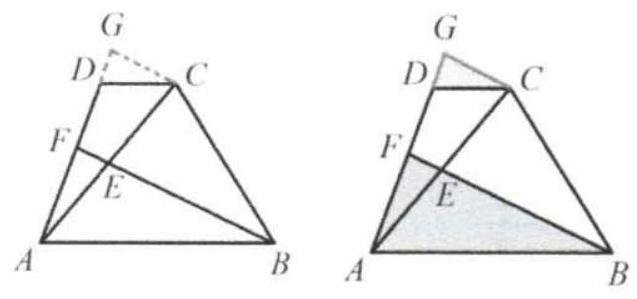
\includegraphics[width=\textwidth]{images/136(3).jpg}
\end{center}

Since \(C G / / E F, A E=E C, A F=F G\). Therefore \(F D=2 D G, \frac{A F}{F D}=\frac{3}{2}\).

\end{document}
